\lstset{
    language=alloy,
    tabsize=4,
    keywordstyle=\color{alloy-keyword}\bfseries,
    commentstyle=\color{alloy-comment},
    stringstyle=\color{alloy-string},
    basicstyle=\small\fontfamily{pcr}\selectfont
}

\section{Signatures}
	\lstinputlisting{../resources/Alloy/alloy_signatures.als}

\newpage
\section{Facts}
	\lstinputlisting{../resources/Alloy/alloy_facts.als}

\newpage
\section{Predicates}
	\lstinputlisting{../resources/Alloy/alloy_predicates.als}

\section{Results}
Executing "Run show for 3" \\
Solver=sat4j Bitwidth=4 MaxSeq=3 SkolemDepth=1 Symmetry=20 \\
5642 vars. 302 primary vars. 13223 clauses. 151ms. \\
Instance found. Predicate is consistent. 49ms. \\

\newpage
\section{Generated World}
\begin{figure}[!ht]
  \centering
  \vspace{0.2cm}
  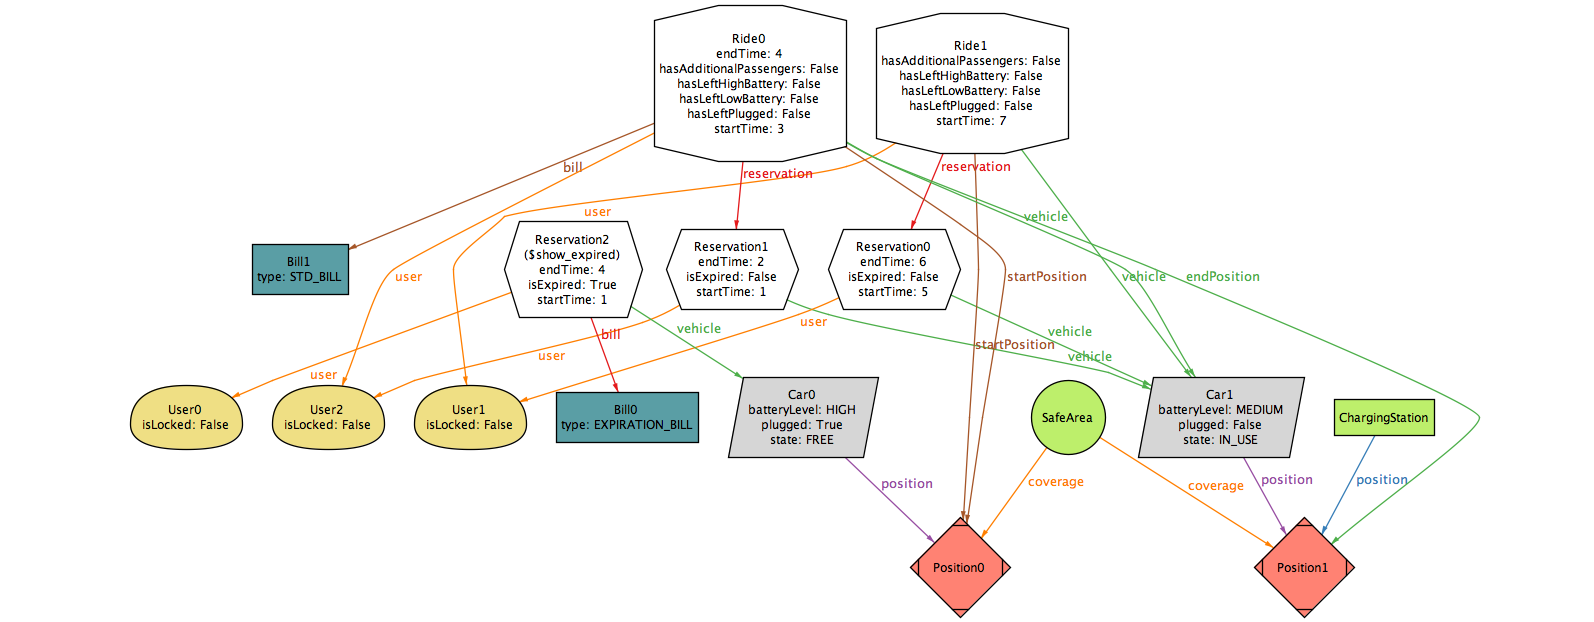
\includegraphics[width=1.4\textwidth, angle=90]{/RASD/alloy_world}\\
  \vspace{0.2cm}
  %\caption{Sequence diagram for the alloy world} 
  \label{fig:alloy_world} 
\end{figure}
